\begin{frame}{\tcv{} ES on noisy environments}%

        \onslide<2->{
        %SpaceInvaders
        \begin{columns}
          \begin{column}{0.45\linewidth}
            \begin{center}
              \begin{figure}
                \centering
                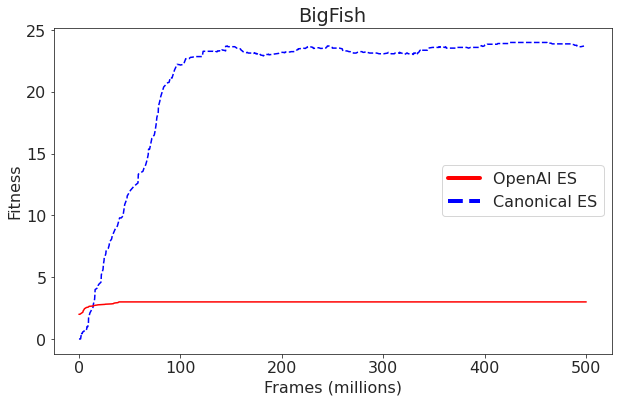
\includegraphics[width=\linewidth]{images/ERL/plots/bigfish_single_1.png}
                \caption{ES on BigFish, same level}
              \end{figure}
            \end{center}
          \end{column}
        }
        \onslide<3->{
          \begin{column}{0.45\linewidth}
            \begin{center}
              \begin{figure}
                  \centering
                  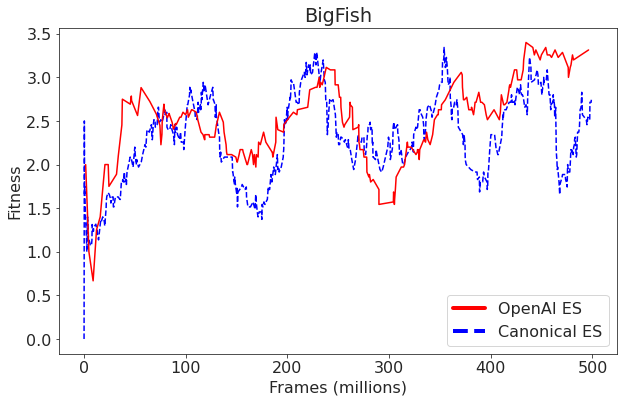
\includegraphics[width=\linewidth]{images/ERL/plots/bigfish_1.png}
                  \caption{ES on BigFish, random level}
              \end{figure}
            \end{center}
          \end{column}
        \end{columns}
        }

      
\end{frame}


\begin{frame}{\tcv{} The \lucie{} selection procedure}%
    \vspace{1em}
    \onslide<2->{%
        \textbf{Objective:} identify the {\color<2>{cyan}\textbf{best $\mu$}} individuals with as {\color<2>{magenta}\textbf{few evaluations}} as possible. \cite{lecarpentierLUCIEEvaluationSelection2022}
    }
    \vspace{1em}
    \begin{figure}
        \def\xmax{10}%
        \def\ymax{5}%
        \def\dx{1.3}%
        \def\hicol{magenta}%
        \def\locol{cyan}%
        \def\elcol{green!60!black}%
        \begin{tikzpicture}[%
                ball/.style={circle,inner sep=0,outer sep=0,minimum width=2mm}
            ]%
            % axis
            \onslide<3->{%
                \draw [stealth-stealth,thick] (0,\ymax) node (yaxis) [above] {} |- (\xmax,0) node (xaxis) [right] {};
                \node[rotate=90] at (-0.4,\ymax-0.7) {\textsc{Fitness}};
                \node[] at (\xmax-1.1,-0.4) {\textsc{Individuals}};
            }
            % individuals
            \onslide<4->{%
                \foreach \x in {1,2,3,4,5}{%
                    \node[ball,fill=black,opacity=1.0] at (\x*\dx,0){};
                }
            }
            \onslide<5>{%
                % mean
                \node[] (i1mean) at (1*\dx,2.5) {};
                \node[red] (mean) at (5,4) {\textbf{Empirical mean:} $\hat{f} = \frac{1}{u} \sumc{k=1}{u} y_k$};
                \draw[red,-stealth] (mean.west) to[out=180,in=0] (i1mean.east);
                % ci
                \node[] (i1ci) at (0.1+1*\dx,2.0) {};
                \node[red] (ci) at (5,0.5) {\textbf{Confidence interval:} $\beta(u,t)$};
                \draw[red,-stealth] (ci.west) to[out=180,in=0] (i1ci.east);
                \roundbracket{0.2+1*\dx}{2.0}{0.45}{red}{0.08}{}{90}% x y width color sidesize thickness rotate
            }
            % t=1 fitnesses
            \onslide<5-7>{%
                \only<5>{%
                    \cifit{1*\dx}{2.5}{1}{black} % x y beta color
                    \cifit{2*\dx}{2.4}{1}{black}
                    \cifit{3*\dx}{2.3}{1}{black}
                    \cifit{4*\dx}{2.3}{1}{black}
                    \cifit{5*\dx}{2.1}{1}{black}
                }
                \only<6->{%
                    \cifit{1*\dx}{2.5}{1}{\hicol} % x y beta color
                    \cifit{2*\dx}{2.4}{1}{\hicol}
                    \cifit{3*\dx}{2.3}{1}{\locol}
                    \cifit{4*\dx}{2.3}{1}{\locol}
                    \cifit{5*\dx}{2.1}{1}{\locol}
                }
            }
            % high low sets
            \onslide<6-8>{%
                \node[] at (1.5*\dx,4) {\color{\hicol}\textsc{High}};
                \node[] at (4.0*\dx,4) {\color{\locol}\textsc{Low}};
                \roundbracket{1.5*\dx}{3.8}{0.6*\dx}{\hicol}{0.1}{}{180}
                \roundbracket{4.0*\dx}{3.8}{1.1*\dx}{\locol}{0.1}{}{180}
            }
            % sampling candidates 1
            \onslide<7>{%
                \node[draw, rounded corners=0.1cm] (sc) at (2.5*\dx,-1) {Sampling candidates};
                \draw[-stealth] (sc.north) to[out=90,in=-90] (2*\dx,-0.1);
                \draw[-stealth] (sc.north) to[out=90,in=-90] (3*\dx,-0.1);
                \node[ball,draw,dashed,thick,minimum width=0.5cm] at (2*\dx,1.4) {};
                \node[ball,draw,dashed,thick,minimum width=0.5cm] at (3*\dx,3.3) {};
            }
            % t=2 fitnesses
            \onslide<8>{%
                \cifit{1*\dx}{2.5}{1}{\hicol} % x y beta color
                \cifit{2*\dx}{2.4}{0.7}{\hicol}
                \cifit{3*\dx}{2.3}{0.7}{\locol}
                \cifit{4*\dx}{2.3}{1}{\locol}
                \cifit{5*\dx}{2.1}{1}{\locol}
            }
            % sampling candidates 2
            \onslide<8>{%
                \node[draw, rounded corners=0.1cm] (sc) at (2.5*\dx,-1) {Sampling candidates};
                \draw[-stealth] (sc.north) to[out=90,in=-90] (1*\dx,-0.1);
                \draw[-stealth] (sc.north) to[out=90,in=-90] (4*\dx,-0.1);
                \node[ball,draw,dashed,thick,minimum width=0.5cm] at (1*\dx,1.5) {};
                \node[ball,draw,dashed,thick,minimum width=0.5cm] at (4*\dx,3.3) {};
            }
            % t=3 fitnesses + stop
            \onslide<9->{%
                % stop
                \draw[thick, dashed] (2*\dx,2.3) -- (6*\dx,2.3);
                \draw[thick, dashed] (3*\dx,2.5) -- (6*\dx,2.5);
                \draw[thick] (6*\dx,2.3-0.5) -- (6*\dx,2.5+0.5);
                \draw[thick,-stealth] (6*\dx,2.3-0.5) -- (6*\dx,2.3);
                \draw[thick,-stealth] (6*\dx,2.5+0.5) -- (6*\dx,2.5);
                \node[] at (6.5*\dx,2.4) {$\leq \epsilon$};
                \node[] at (6.5*\dx,3.4) {Stopping Criterion:};
                % sets
                \node[] at (1.5*\dx,4.9) {\color{\hicol}\textsc{High}};
                \node[] at (4.0*\dx,4.9) {\color{\locol}\textsc{Low}};
                \roundbracket{1.5*\dx}{4.7}{0.6*\dx}{\hicol}{0.1}{}{180}
                \roundbracket{4.0*\dx}{4.7}{1.1*\dx}{\locol}{0.1}{}{180}
                % fit
                \cifit{1*\dx}{3.5}{1}{\hicol} % x y beta color
                \cifit{2*\dx}{2.8}{0.5}{\hicol}
                \cifit{3*\dx}{1.8}{0.7}{\locol}
                \cifit{4*\dx}{1.5}{0.5}{\locol}
                \cifit{5*\dx}{1.2}{0.9}{\locol}
                % elite
                \node[ball,fill=\elcol] at (1*\dx,0){};
                \node[ball,fill=\elcol] at (2*\dx,0){};
                \node[] at (1.5*\dx,-0.5) {\color{\elcol}\textsc{Elite}};
                \roundbracket{1.5*\dx}{-0.3}{0.6*\dx}{\elcol}{0.1}{}{0}
            }
        \end{tikzpicture}%
    \end{figure}
\end{frame}

\begin{frame}{\tcv{} \onemax{} and \leadingones{}}%
    \onslide<2->{
    \def\figwidth{0.28\linewidth}%
    \def\xleg{\# Evaluations $\times 1000$}%
    \def\yleg{Fitness}%
    \begin{textblock*}{2cm}(0cm,0.9cm) % {block width} (coords)
        $\%$noise
    \end{textblock*}
    \begin{table}%[h!]
        \centering
        \begin{tabular}{ccccc}
            && $0\%$ & $100\%$ & $200\%$ \\
            \raisebox{3\normalbaselineskip}[0pt][0pt]{\rotatebox[origin=c]{90}{\onemax{}}} &
            \raisebox{3\normalbaselineskip}[1cm][0cm]{\rotatebox[origin=c]{90}{\vspace{1cm}\yleg}}&
            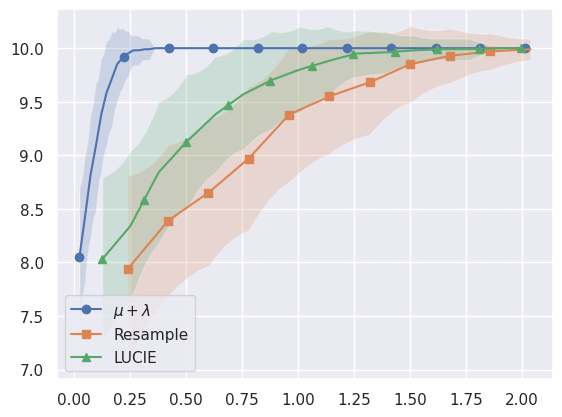
\includegraphics[width=\figwidth]{images/LUCIE/onemax/uniform/all_ones_0_u_fitness.png} &
            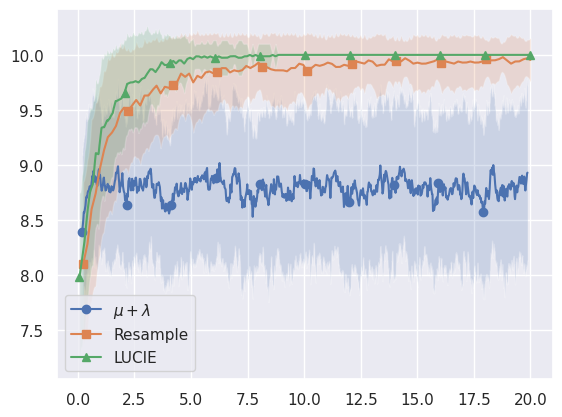
\includegraphics[width=\figwidth]{images/LUCIE/onemax/uniform/all_ones_100_u_fitness.png} &
            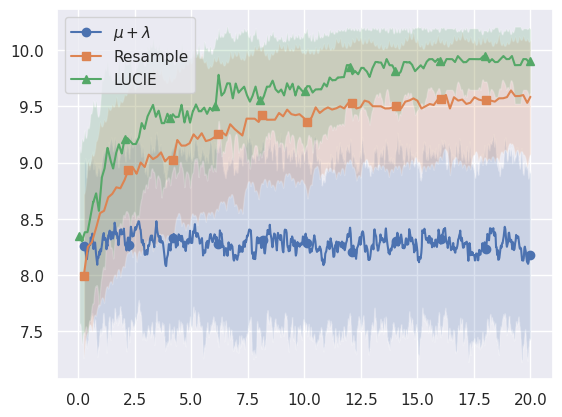
\includegraphics[width=\figwidth]{images/LUCIE/onemax/uniform/all_ones_200_u_fitness.png}\\
            \raisebox{3\normalbaselineskip}[0pt][0pt]{\rotatebox[origin=c]{90}{\leadingones{}}} &
            \raisebox{3\normalbaselineskip}[1cm][0cm]{\rotatebox[origin=c]{90}{\vspace{1cm}\yleg}}&
            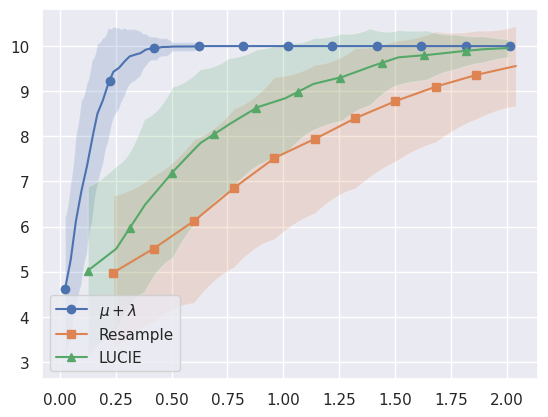
\includegraphics[width=\figwidth]{images/LUCIE/leadingones/uniform/leading_ones_0_u_fitness.png} &
            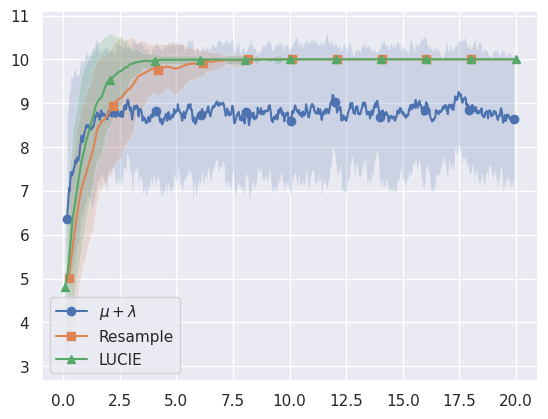
\includegraphics[width=\figwidth]{images/LUCIE/leadingones/uniform/leading_ones_100_u_fitness.png} &
            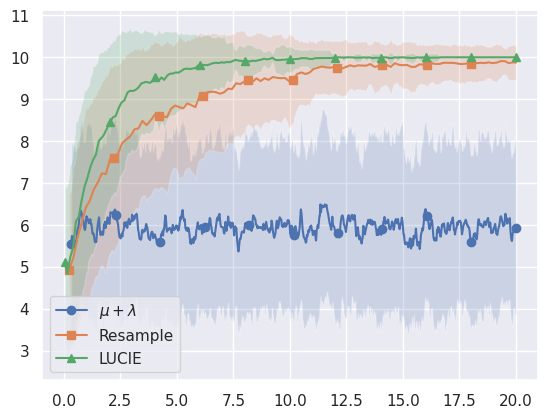
\includegraphics[width=\figwidth]{images/LUCIE/leadingones/uniform/leading_ones_200_u_fitness.png}\\
            &&\xleg&\xleg&\xleg
        \end{tabular}
%			\caption{Results for \onemax{} and \leadingones{} under posterior uniform noise.}
%			\label{table:toy-exp-uniform}
    \end{table}
    }
\end{frame}

% LUCIE ES
\begin{frame}{\tcv{} \lucie{} for Evolution Strategies}%
    \begin{figure}
        
    \tikzset{every picture/.style={line width=0.75pt}} %set default line width to 0.75pt        

    \begin{tikzpicture}[x=0.75pt,y=0.75pt,yscale=-1,xscale=1]
    %uncomment if require: \path (0,300); %set diagram left start at 0, and has height of 300
        \onslide<2->{
        %Shape: Axis 2D [id:dp6438436813949673] 
        \draw  (61.09,246.2) -- (495.88,246.2)(104.57,34.7) -- (104.57,269.7) (488.88,241.2) -- (495.88,246.2) -- (488.88,251.2) (99.57,41.7) -- (104.57,34.7) -- (109.57,41.7)  ;
        % Text Node
        \draw (503.2,237.2) node [anchor=north west][inner sep=0.75pt]  [font=\small]  {$rank$};
        % Text Node
        \draw (114.8,37) node [anchor=north west][inner sep=0.75pt]  [font=\small]  {$weight$};
        }

        \onslide<3->{
        %Straight Lines [id:da7596112643907376] 
        \draw [color={rgb, 255:red, 255; green, 0; blue, 0 }  ,draw opacity=1 ]   (104.69,106.9) -- (235.87,106.9) -- (236.59,246.1) -- (465.09,246.1) ;
        \draw (85.2,93) node [anchor=north west][inner sep=0.75pt]  [font=\scriptsize,color={rgb, 255:red, 255; green, 2; blue, 33 }  ,opacity=1 ]  {$\frac{1}{\mu }$};
        \draw (370.87,67.67) node [anchor=west] [inner sep=0.75pt]  [color={rgb, 255:red, 255; green, 0; blue, 0 }  ,opacity=1 ] [align=left] {Split};
        }

        \onslide<4->{
        %Curve Lines [id:da6394141615756642] 
        \draw [color={rgb, 255:red, 97; green, 174; blue, 9 }  ,draw opacity=1 ]   (105.2,78.2) .. controls (115.09,103.35) and (186.69,191.75) .. (260.69,214.15) .. controls (334.69,236.55) and (435.15,245.18) .. (465.09,246.1) ;
        \draw (370.6,88.73) node [anchor=west] [inner sep=0.75pt]  [color={rgb, 255:red, 97; green, 174; blue, 9 }  ,opacity=1 ] [align=left] {Rank};
        }

    \end{tikzpicture}

    \end{figure}
\end{frame}

\begin{frame}{\tcv{} Importance Mixing for LUCI ES}%
    \begin{figure}

    \tikzset{every picture/.style={line width=0.75pt}} %set default line width to 0.75pt        

    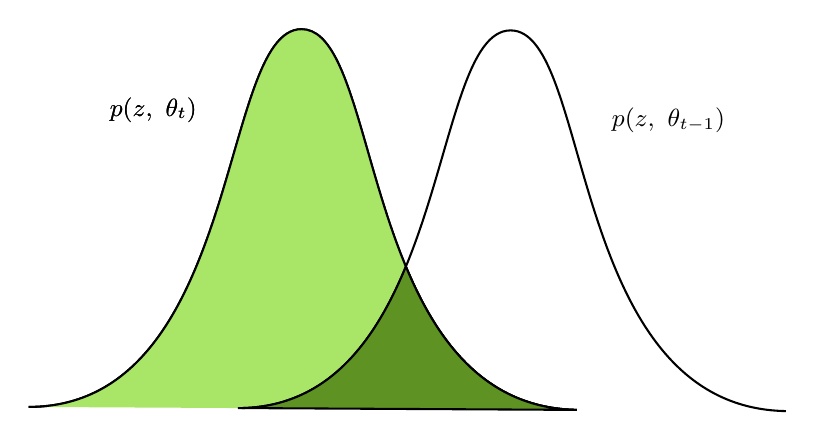
\begin{tikzpicture}[x=0.75pt,y=0.75pt,yscale=-1,xscale=1]
    %uncomment if require: \path (0,300); %set diagram left start at 0, and has height of 300
    
        \only<3>{
        %Shape: Boxed Bezier Curve [id:dp19284355666403086] 
        \draw    (163.42,256.57) .. controls (266.14,256.57) and (255.08,74.89) .. (294.76,74.57) .. controls (323.56,74.35) and (324.97,170.2) .. (363.9,223.42) .. controls (378.6,243.51) and (398.64,257.52) .. (427.52,258) ;
        \draw (201.02,105.96) node [anchor=north west][inner sep=0.75pt]  [font=\small]  {$p( z,\ \theta _{t})$};   
        }
        \onslide<4->{
        %Shape: Boxed Bezier Curve [id:dp19284355666403086] 
        \draw [fill={rgb, 255:red, 169; green, 229; blue, 103 }  ,fill opacity=1 ]   (163.42,256.57) .. controls (266.14,256.57) and (255.08,74.89) .. (294.76,74.57) .. controls (323.56,74.35) and (324.97,170.2) .. (363.9,223.42) .. controls (378.6,243.51) and (398.64,257.52) .. (427.52,258) ;
        \draw (201.02,105.96) node [anchor=north west][inner sep=0.75pt]  [font=\small]  {$p( z,\ \theta _{t})$};   
        }

        \onslide<2->{
        %Shape: Boxed Bezier Curve [id:dp5389195998778902] 
        \draw    (264.16,257.15) .. controls (366.88,257.15) and (355.82,75.47) .. (395.5,75.16) .. controls (435.18,74.84) and (422.87,256.84) .. (528.26,258.58) ;
        \draw (442.91,110.85) node [anchor=north west][inner sep=0.75pt]  [font=\small]  {$p( z,\ \theta _{t-1})$};
        }
        \onslide<4->{
        %Shape: Path Data [id:dp639977105939747] 
        \draw  [fill={rgb, 255:red, 94; green, 147; blue, 36 }  ,fill opacity=1 ] (363.9,223.42) .. controls (378.6,243.51) and (398.64,257.52) .. (427.52,258) -- (266.2,257.12) .. controls (307.63,256.14) and (330.18,225.11) .. (345.13,188.95) .. controls (350.31,201.36) and (356.41,213.18) .. (363.9,223.42) -- cycle ;
        }

    \end{tikzpicture}

    \end{figure}
\end{frame}

